\subsection{Triangle Split}
A triangle is a planar object, and is representing a possibly non-planar
portion of a surface. Any triangle, with area $A_T$, in the
discretization can have at most the same area as the portion of the
surface which it represents, $A_S$. Therefore, the representation
deficit for a triangle, $RD_T$, is defined as $RD_T = \frac{A_S -
A_T}{A_T}$. Note that the areas are calculated in ${\mathbb R}^3$. The
difference in surface area, $\left(A_S - A_T\right)$, is normalized by
$A_T$ so that the result is scale independent. Also, this is a
representation {\it deficit} since $A_S \ge A_T$ is always true.

In order to apply the above definition of representation deficit to a
mesh generation, a replacement for $A_S$ must be determined since the
area of the surface represented by $A_S$ is not always able to be
determined---or, most often, the area calculation is impractical.
Generally, in order to reduce the representation deficit for a triangle
the triangle is split by inserting an interior point. Any point that is
inserted into the interior of the triangle would decrease the
representation deficit---or at worst it will remain the same. However,
the determination of where to split the triangle should be done in such
a way that the representation deficit is minimized. This strategy of
refinement, refining each triangle in such a way that the representation
deficit is locally minimized, would take advantage of the optimal
substructure the discrete topology.

\begin{figure}[h!]
  \center{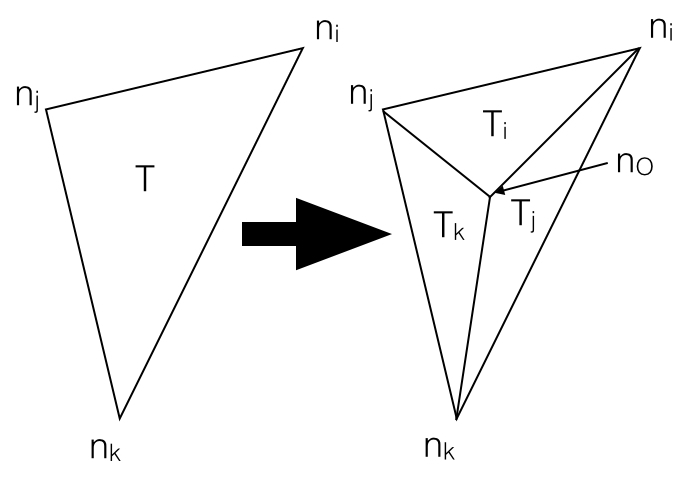
\includegraphics[height=1.4in]
    {Figures/TriangleSplit.jpg}}
  \caption{Triangle Split}
\end{figure}

The process of determining where to split a triangle is defined here by
a locally optimizing an objective function defined for a triangle: Let
$S(u,v)$ be a parameterized surface, $D$ be be a discretization of the
surface, and $T$ be a triangle (included in $D$) defined by an ordered
tuple of nodes, $\left(n_i, n_j, n_k\right)$. These nodes are ordered
such that the triangle normal is positive. Specifically, if $\vec{V_0} =
\left\{n_j - n_i \right\}$ and $\vec{V_1} = \left\{n_k - n_i\right\}$
then the triangle normal, $N_T = \vec{V_0} \times \vec{V_1}$, is
positive. Note that a two-dimensional cross-product (or two-dimensional
curl) is a scalar quantity. Additionally, let a node on the interior of
$T$ be defined as $n_O$. The four nodes, $n_i$, $n_j$, $n_k$, and $n_O$
define three triangles, $T_i\left(n_i,n_j,n_0\right), T_j\left(n_j, n_k,
n_0\right), T_k\left(n_k, n_i, n_0\right)$. If $A(T)$ is a function
that calculates the area of a triangle in $\left(x,y,z\right)$ space,
then the optimization problem for finding the optimal position for $n_0$
in $T$ is defined as:

\begin{eqnarray*}
\begin{array}{rcl}
\underset{n_O}{\text{minimize}} \ O(T) & = & - \frac{A\left(T_i\right) + A\left(T_j\right) + A\left(T_k\right) }{ A\left(T\right) }\\
\text{subject to} \ N_{T_i} & > & 0 \\
N_{T_j} & > & 0 \\ 
N_{T_k} & > & 0. \\
\end{array}
\end{eqnarray*}

It should be noted that this definition of representation deficit would
be difficult to derive or express for a topological entity other than a
triangle. This is due to the inherent ambiguity in the definition of not
only the surface area, but also the surface representation of (possibly)
non-planar elements, e.g. non-planar, or skew, quadrilateral. [MORE
POSSIBLY]
